\subsection{Introducción a riesgos estáticos}
En este punto se analiza la siguiente tabla de verdad:
\begin{table}[H]
\centering
\begin{tabular}{ccccc}
\hline
\textbf{a} & \textbf{b} & \textbf{c} &  & \textbf{Y} \\
\hline
0          & 0          & 0          &  & 0         \\
0          & 0          & 1          &  & 1         \\
0          & 1          & 0          &  & 1         \\
0          & 1          & 1          &  & 1         \\
1          & 0          & 0          &  & 0         \\
1          & 0          & 1          &  & 1         \\
1          & 1          & 0          &  & 0         \\
1          & 1          & 1          &  & 0         \\
\hline
\end{tabular}
\caption{Tabla de verdad analizada.}
\label{tabla:verdad}
\end{table}

Para ello, se vale del uso de un mapa de Karnaugh. De esta forma se encuentra su mínima expresión, la cuál se decidió expresar en minterminos.

\begin{figure}[H]
\begin{centering}
    \begin{Karnaughvuit}
        \minterms{1,2,3,5}
        \maxterms{0,4,6,7}
        
        \implicant{3}{2}{yellow}
        \implicant{1}{5}{green}   
    \end{Karnaughvuit}
\par\end{centering}
\centering
\caption{Mapa de Karnaugh de la Tabla (\ref{tabla:verdad}).}
\label{fig:karsinc}
\end{figure}

Es así, que observando la Figura (\ref{fig:karsinc}), se llega a la expresión:
\begin{equation}
	Y \left( a,b,c \right) = \bar{b} c + \bar{a} b
	\label{equ:karsinc}
\end{equation}

Una forma de representar (\ref{equ:karsinc}) se muestra en la Figura (\ref{fig:cirsinc}).

\begin{figure}[H]
\begin{center}
\begin{circuitikz}
	\node [american and port](A2){};
	\draw (A2.bin 2) node[ocirc](){};	
	\draw (A2.in 2) to[short] ++(-2,0) to[short] ++(0,4) node[circ, label=north:$b$](b){};
	\draw (A2.in 1) to[short] ++(-1,0) to[short] ++(0,3.45) node[circ, label=north:$c$](c){};
	\draw (A2) to[open] ++(0,2) node[american and port](A1){};
	\draw (A1.bin 1) node[ocirc](){};
	\draw (A1.in 2) to[short, -*] ++(-2,0);
	\draw (A1.in 1) to[short] ++(-3,0) to[short] ++(0,1.5) node[circ, label=north:$a$](a){};
	\draw (A1.out) to[short] ++(0,-0.75) node[american or port, anchor=in 1](O){};
	\draw (A2.out) |- (O.in 2);
	\draw (O.out) to[short] ++(0.5,0) node[circ, label=$y$](y){};
	\draw (A1.out) node[label=right:$\alpha$](){};
	\draw (A2.out) node[label=right:$\beta$](){};
\end{circuitikz}
\caption{Circuito posible que representa a (\ref{equ:karsinc}).}
\label{fig:cirsinc}
\end{center}
\end{figure}

Desde una perspectiva sincrónica, este circuito no presenta ningún problema, ya que las señales existentes se propagan al mismo tiempo, si ningún tipo de demora en cada compuerta. Pero desde una perspectiva asincrónica no ocurre lo mismo.

Se analiza el caso en el cual $a = 0$ y $b = c = 1$, siendo entonces $Y = 1$. Si se permite que $b$ cambie de 1 a 0, $Y$ debe seguir siendo 1. Si se considera la demora existente en la propagación de una señal a través de una compuerta, el cambio de $b$ puede llegar a ser visto en el nodo $\alpha$ antes que en el $\beta$, ya que para llegar a este último, la señal debe atravesar una compuerta más que para llegar al primero (la compuerta NOT previa a la AND). Por lo tanto, en este caso existe la posibilidad de obtener $\alpha = 0$ y $\beta = 0$, haciendo que $Y = 0$. Esto es lo que se conoce como un riesgo estático, los cuales son visibles cuando la salida debe mantenerse constante frente a un cambio de una de las variables de entrada, pero en vez de ser así, la salida varía momentáneamente para luego volver al valor debido.

\begin{figure}[H]
\begin{center}
\begin{circuitikz}
	\node [label=left:$1$](1){};
	\draw (1) to[open] ++(0.5,0) to[short] ++(1,0) to[short] ++(0,-1) to[short] ++(0.5,0) to[short] ++(0,1) to[short] ++(2,0);
	\draw (1) to[open] ++(0,-1) node[label=left:$0$](0){};
	
	\draw (0) to[open] ++(5,0) to[short] ++(1,0) to[short] ++(0,1) to[short] ++(0.5,0)to[short] ++(0,-1) to[short] ++(2,0);
\end{circuitikz}
\caption{Salida de un circuito frente a un error de riesgo estático.}
\label{fig:riesgosestaticos}
\end{center}
\end{figure}

Es posible detectar un un error potencial observando el mapa de Karnaugh, ya que en cualquier lugar que se encuentre un par de 1s adyacentes que no sean cubiertos por un grupo de minterminos, puede existir un error como el mencionado (de la misma forma ocurre con los 0s y los maxterminos). Por lo tanto, agregando algún nuevo conjunto que incluya dicho par adyacente, se evita que exista un error de transición ya que dicho conjunto se encuentra incluido en un grupo.\footnote{S. Brown and Z. Vranesic, Fundamentals of digital logic with verilog design, 3er ed. New York: McGraw-Hill, 2002.}

Por lo tanto, considerando todo lo dicho se vuelve a considerar el mapa de Karnaugh de la Tabla (\ref{tabla:verdad}), pero esta vez tomando un grupo adicional, representado en rojo:
\begin{figure}[H]
\begin{centering}
    \begin{Karnaughvuit}
        \minterms{1,2,3,5}
        \maxterms{0,4,6,7}
        
        \implicant{3}{2}{yellow}
        \implicant{1}{5}{green}
        \implicant{1}{3}{red}        
    \end{Karnaughvuit}
\par\end{centering}
\centering
\caption{Mapa de Karnaugh en un modelo asincrónico.}
\label{fig:karasinc}
\end{figure}

La consideración presentada en la Figura (\ref{fig:karasinc}) conduce a una nueva expresión, siendo esta:
\begin{equation}
	Y \left( a,b,c \right) = \bar{b} c + \bar{a} b + \bar{a} c
	\label{equ:karasinc}
\end{equation}

De la misma forma que antes, se busca representar la ecuación hallada a partir del mapa de Karnaugh mediante un circuito lógico. Esto conduce al representado en la Figura (\ref{fig:cirasinc}).

\begin{figure}[H]
\begin{center}
\begin{circuitikz}
	\node [american and port](A2){};
	\draw (A2.bin 2) node[ocirc](){};	
	\draw (A2.in 2) to[short] ++(-2,0) to[short] ++(0,4) node[circ, label=north:$b$](b){};
	\draw (A2.in 1) to[short, -*] ++(-1,0) to[short] ++(0,3.45) node[circ, label=north:$c$](c){};
	\draw (A2) to[open] ++(0,2) node[american and port](A1){};
	\draw (A1.bin 1) node[ocirc](){};
	\draw (A1.in 2) to[short, -*] ++(-2,0);
	\draw (A1.in 1) to[short, -*] ++(-3,0) to[short] ++(0,1.5) node[circ, label=north:$a$](a){};
	\draw (A2.out) to[short] ++(1,0) node[american or port, number inputs=3, anchor=in 2](O){};
	\draw (A2.out) |- (O.in 2);
	\draw (O.out) to[short] ++(0.5,0) node[circ, label=$y$](y){};
	\draw (A2) to[open] ++(0,-2) node[american and port](A3){};
	\draw (A3.bin 2) node[ocirc](){};
	\draw (a) |- (A3.in 2);
	\draw (c) |- (A3.in 1);
	\draw (A1.out) |- (O.in 1);
	\draw (A3.out) |- (O.in 3);
\end{circuitikz}
\caption{Circuito posible que representa a (\ref{equ:karasinc}).}
\label{fig:cirasinc}
\end{center}
\end{figure}

\subsection{Desarrollo del circuito}

Se implementó el circuito de la Figura (\ref{fig:cirasinc}) en un PCB. Para ello se valió del uso de las compuertas \href{http://www.ti.com/lit/ds/symlink/sn74hc04.pdf}{SN74HC04}, \href{http://www.ti.com/lit/ds/symlink/sn74hc08.pdf}{SN74HC08} y \href{http://www.ti.com/lit/ds/symlink/sn74hc32.pdf}{SN74HC32}. Para poder realizar las mediciones adecuadas, y debido a que no se contaba con una compuerta OR de tres entradas, se decidió implementar en una primera instancia lo observado en la Figura (\ref{fig:cirsinc}) (es decir, el circuito que representa a $\bar{b} c + \bar{a} b$), la cual se encuentra conectada a una bornera para poder medirla y también a otra compuerta OR, cuya segunda entrada es la resultante del termino faltante ($\bar{a} c$), la cual se encuentra conectada a otra bornera. De esta forma se puede medir tanto el circuito sin la implementación de la solución del glitch y como con dicha implementación.

\subsection{Mediciones}

Se procede a simular la situación ejemplificada previamente, es decir con  $a = 0$ y $c = 1$, alternando el valor de $b$ entre $0$ y $1$. Dicha variación se simula utilizando un generador de ondas cuadradas, el cuál oscila entre $0 \ V$ y $5 \ V$. Observando tanto la entrada como las dos salidas previamente mencionadas, se obtiene lo siguiente: 
\begin{figure}[H]
\centering
	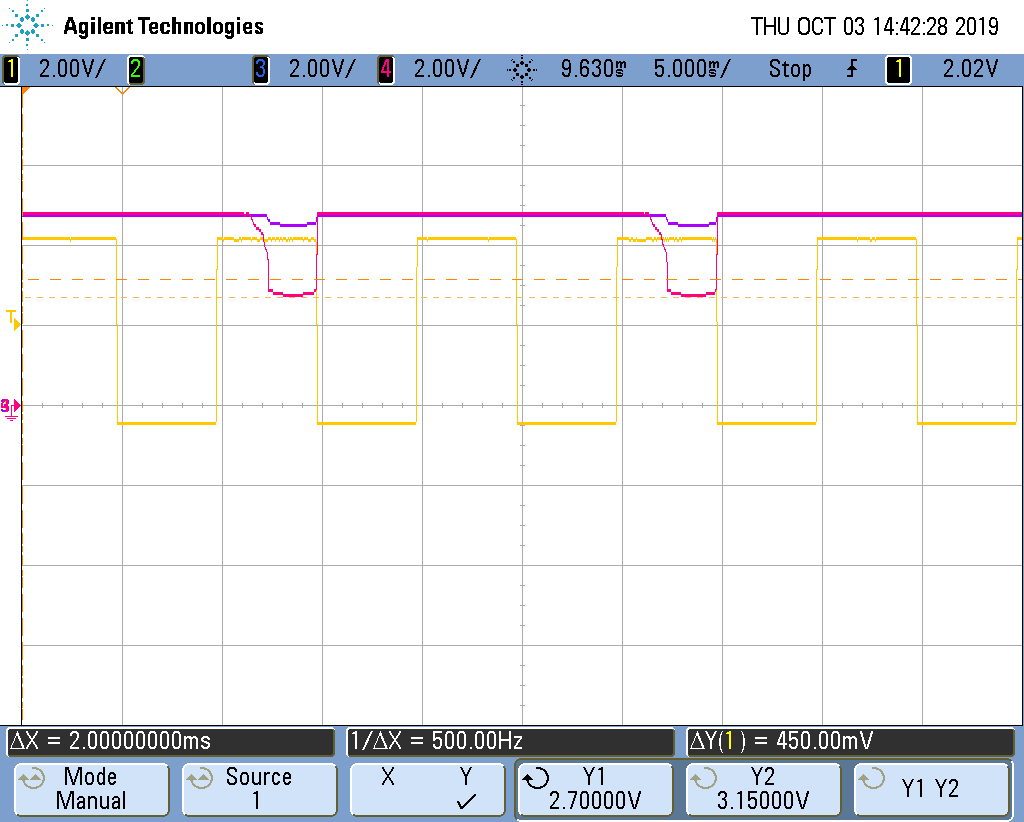
\includegraphics[width=0.8\textwidth, trim = {0 0 0 2cm},clip]{ImagenesEjercicio3/scope_5.png}
	\caption{Salida con glitch (rosa) y sin glitch (violeta) variando $b$ (amarillo).}
	\label{fig:medicion}
\end{figure}

Por un lado se observa de la figura anterior como la salida varía en función de la entrada. Si bien la señal que no posee la solución al glitch (señal rosada) no decae por completo a un cero lógico, esta posee una variación importante, la cual vale destacar. Dicha variación coloca la tensión a la salida de la primer compuerta OR por debajo de los $3.15 \ V$, valor que, según la tecnología adoptada, es menor a la tensión $V_{OH}$, por ende, este valor deja de ser considerado como un uno lógico. Por otro lado, se denota que la señal que sí posee dicha solución (señal violeta) también posee una variación, la cual no es de importancia ya que se sigue manteniendo por encima de $V_{IH}$, de forma el valor lógico de esta salida no varía.